\chapter{Concept}
\label{ch:Concept}

A methodologist first annotates the reactions of a consistency specification with the features they belong to.
A derivation step then reduces the annotated specification to the rules of a single configuration.
Everything built with those rules is consistent under them, whereas a V-SUM that was persisted under an earlier configuration is not.
The second part of the chapter therefore describes the migration that brings such a V-SUM to the rules it is loaded with.
The feature model, the nine configurations and the library example are introduced in \autoref{ch:RunningExample}.
The approach is stated independently of the tool that realizes it and of the metamodels it is applied to, a claim that \textbf{M5.1} and \textbf{M5.2} put to the test.
The realization is described in \autoref{ch:Implementation}, and \autoref{ch:Evaluation} reports the measurements defined by the metrics of \autoref{sec:Introduction:ResearchGoals}.
Each part of this chapter names the metrics that judge it.

\section{Feature annotations}
\label{sec:Concept:FeatureAnnotations}

A consistency specification written in the Reactions Language fixes one mapping between the involved metamodels.
Several mappings are often defensible.
A UML class can be realized as a Java class, as an interface or as an enumeration, and the methodologist has to commit to one of these alternatives.
Supporting a second project convention then requires a second copy of the specification, in which every correction to a shared rule has to be applied again.
Treating the specification as the asset base of a software product line removes that commitment, as described in \autoref{sec:Foundations:SoftwareProductLines}.
The reactions of all variants form one 150\% rule set.
Every reaction of that rule set carries an annotation with the feature it belongs to, which makes the variability annotative \cite{kaestner2008granularity}.
A feature model states which combinations of features are valid, whereas a configuration selects the rules of one variant \cite{apel2013software,czarnecki2005mapping}.
\textbf{M1.2} counts the files that an added or changed variant costs under either arrangement.

\subsection{Annotating reactions}
\label{sec:Concept:FeatureAnnotations:AnnotatingReactions}

An annotation is attached to a reaction and names the feature the reaction belongs to.
The reaction in \autoref{listing:annotated-reaction} realizes an inserted UML class as a Java interface.
It belongs to \textit{ClassCreation.Interface}, one of the three alternatives of \textit{ClassCreation}, and replaces \autoref{listing:existing-reaction} of the running example, which belongs to \textit{ClassCreation.Class}.
The feature names are those of the feature model in \autoref{sec:RunningExample:FeaturesAndConfigurations}, although the annotation does not check that the name it carries exists there.

\lstinputlisting[frame=single, caption={Reaction annotated with a feature}, label=listing:annotated-reaction, numbers=left, float=htbp, language=reactions]{examples/umlClassInsertedAnnotation.reactions}

An annotation carries exactly one feature name and admits neither boolean expressions over features nor nesting.
The restriction costs no expressiveness, because behavior shared by two features is expressed by a routine that the reactions of both features call.
A conjunction of features would merely restate in the asset base what the feature model already declares.
Routines carry no annotation at all.
Since they have no trigger, they belong to a feature only through the reactions that reach them, which is the property the derivation described in \autoref{sec:Concept:FeatureAnnotations:RuleSetDerivation} relies on.

\lstinputlisting[frame=single, caption={Routine selected by \textit{ClassCreation.Interface}}, label=listing:chosen-routine, numbers=left, float=htbp, language=reactions]{examples/createJavaInterfaceFromClass.reactions}
\lstinputlisting[frame=single, caption={Routine selected by \textit{ClassCreation.Enum}}, label=listing:possible-routine, numbers=left, float=htbp, language=reactions]{examples/createJavaEnumFromClass.reactions}

The two alternatives of \textit{ClassCreation} differ in the routine their reactions call.
The routine in \autoref{listing:chosen-routine} creates a Java interface and is reached only through the reaction of \autoref{listing:annotated-reaction}.
The routine in \autoref{listing:possible-routine}, by contrast, creates an enumeration and is reached only through the corresponding reaction of \textit{ClassCreation.Enum}.
Both routines establish a correspondence between the UML class and the Java classifier they create.
That correspondence is the record of the derivation which the migration later reads.
\textbf{M1.3} records how much of the original rule set had to be changed to become a 150\% rule set.

\subsection{Rule set derivation}
\label{sec:Concept:FeatureAnnotations:RuleSetDerivation}

The derivation takes the 150\% rule set and one configuration and writes the rules of that configuration.
A reaction is kept if the configuration selects the feature its annotation names.
A reaction without an annotation belongs to no feature and could never be selected, so carrying one is a well-formed condition on a 150\% rule set rather than a consequence of the derivation.
The routines a reaction calls are kept with it, together with the routines those call in turn, whereas what no kept reaction reaches is left out.
This is how the routines of an unselected alternative disappear, although no annotation ever mentioned them.

Features that the feature model declares mandatory are part of every valid configuration, and their reactions appear in every derived rule set.
Only the reactions of the optional features and of the alternative groups differ between two configurations.
Two derived rule sets of the library example therefore overlap in the large majority of their rules.
The result of a derivation is an ordinary rule set without annotations.
Since the compiler of the Reactions Language processes it like any handwritten one, nothing downstream of the derivation has to know that features exist.
The derivation of config1 and config7 of the library example from the same 150\% rule set is shown in \autoref{fig:preprocessor-flow}.

\begin{figure}[htbp]
    \centering
    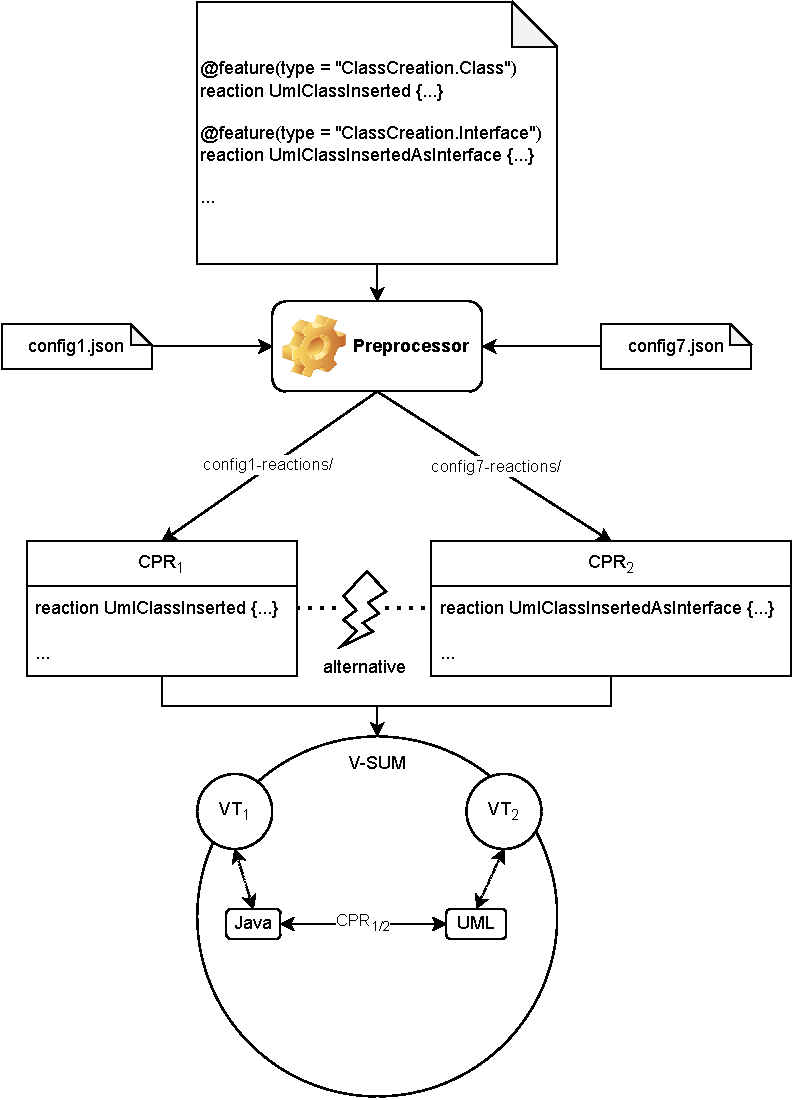
\includegraphics[width=\linewidth,height=0.85\textheight,keepaspectratio]{examples/library/preprocessor.pdf}
    \caption{Derivation of the configurations config1 and config7 of the library example from the annotated reactions.}
    \label{fig:preprocessor-flow}
\end{figure}

The derivation does not check the configuration it is given.
A configuration that violates the feature model by selecting two alternatives of \textit{ClassCreation} yields a rule set with two reactions on the same trigger rather than an error.
Ensuring validity is therefore a duty of the methodologist, who has the feature model to check a configuration against.

One property of the annotation matters beyond this section.
The annotation is not part of the abstract syntax of a reaction, and a kept reaction is written out unchanged apart from the annotation itself.
Two configurations therefore differ in which rules exist, never in what a rule they share does.
That property is taken up again in \autoref{sec:Concept:Migration:SelectiveMigration:SemanticHashes}.
\textbf{M1.1} compares the size of the 150\% rule set against the sum of the configurations it replaces.
\textbf{M1.4} checks that every derived configuration produces compilable code and passes the tests of the case study, whereas \textbf{M1.5} measures what the derivation adds to building and testing a configuration.

\subsection{Binding time}
\label{sec:Concept:FeatureAnnotations:BindingTime}

A feature annotation binds a decision when the rule set is derived.
Vitruvius already contains a second kind of variability, which binds later.
A reaction that lacks the information to proceed can ask the developer at runtime, as described in \autoref{sec:Foundations:Vitruvius}.
Both kinds produce several possible outcomes for one change, yet they do so at different moments and at a different granularity.
A configuration decides once for a whole rule set and is recorded in a file, whereas a dialog decides per element and can be answered differently in two runs of the same rule set.
Only the first of the two makes a run reproducible.

The running example contains such a dialog.
The collection type a Java field receives when the upper multiplicity of a UML property changes is chosen by the developer, as shown in \autoref{listing:existing-user-interaction}.
This work does not express that choice as a feature, so the dialog is present in the 150\% rule set and in all nine derived configurations.
A derived rule set is consequently free of compile-time variability but not of runtime decisions.
A migration has to answer such a dialog without a person present.
It records the interactions a run requires and supplies a fixed answer to each of them.
A question that cannot be answered safely aborts the run, so that no migration rests on an answer that was never given.
What moving such a decision to derivation time would require is discussed in \autoref{ch:FutureWork}.

\section{Migration}
\label{sec:Concept:Migration}

A derived rule set keeps a V-SUM consistent that is built with it.
A V-SUM that already exists was built with a different rule set, and nothing in it records that fact.
A persisted V-SUM holds its models, the correspondences between their elements and the identifiers of those elements, yet it holds no information about the rules that produced any of it \cite{vitruviusGithub}.
Loading it with a new rule set therefore succeeds and leaves the state untouched.
Only the changes made from that point on are propagated by the new rules.
Everything the old rules derived stays as it is, whether the new rules would derive it or not.
The result is a V-SUM that is consistent under neither rule set.
\textbf{M3.1} classifies the inconsistencies that arise in this situation.

Migration closes that gap.
It takes a persisted V-SUM and a rule set and leaves a V-SUM that is consistent under the rules it was given, keeping as much of the existing state as those rules allow.
Two ways of doing so are described here.
The full migration of \autoref{sec:Concept:Migration:FullMigration} keeps one model and derives everything else from it again, without asking what changed in the rule set.
The selective migration of \autoref{sec:Concept:Migration:SelectiveMigration} first establishes which rules changed and then restricts the work to the elements those rules apply to.
Since both leave behind content that no rule derives, the preservation step of \autoref{sec:Concept:Migration:Preservation} collects that content afterward.
\textbf{M2.1} compares a migrated V-SUM against the state the new rules derive from scratch.
\textbf{M2.2} checks that the migrated code still compiles, and \textbf{M2.4} whether migrating back reproduces the original V-SUM.

\subsection{Full migration}
\label{sec:Concept:Migration:FullMigration}

The full migration rests on the single assumption that one model of the V-SUM is authoritative and that every other model can be produced from it.
That model is the dominant model, whereas the models produced from it are the derived models.
Which model dominates is the only decision the full migration makes, and the three ways of making it are described below.
The procedure and those three strategies are shown in \autoref{fig:full-migration}.

\begin{figure}[htbp]
    \centering
    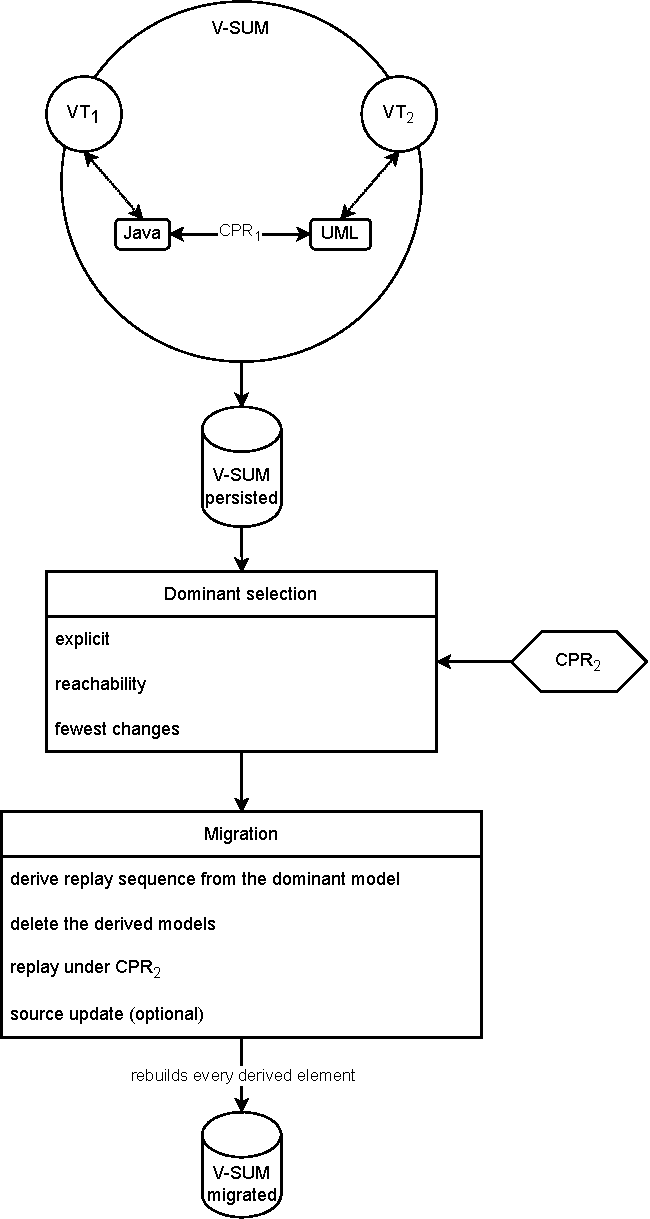
\includegraphics[width=\linewidth,height=0.85\textheight,keepaspectratio]{examples/library/migration.pdf}
    \caption{Full migration of a persisted V-SUM, from the selection of the dominant model to the derivation of the remaining models under the new rules.}
    \label{fig:full-migration}
\end{figure}

Once the dominant model is chosen, the derived models are discarded and produced again from it under the new rules.
Nothing of the old derived state is reused, which makes the procedure a re-derivation rather than a repair.
The new rules see the dominant model as a model that was not present before and derive the other models from it.

The dominant model is kept as a snapshot before the derived side is discarded.
That snapshot is what replaying the history of the V-SUM would leave behind, expressed as state rather than as a sequence of changes.
Reconstructing such a sequence is unnecessary, since reactions respond to the changes a commit produces and committing a whole model at once produces the insertions that build it.
The two are equivalent in what the migration needs from them, namely the state the new rules are shown.
A recorded history could nevertheless contain intermediate steps, such as a rename after an insertion, that the snapshot does not reproduce as changes.

The assumption that one model suffices holds only where the propagations of that model reach every other model of the V-SUM.
Where they do not, further models are taken as dominant until every model is covered, so the decision is in general a set of dominant models rather than a single one.
Every model that is not dominant is derived again.

An optional source update follows the derivation.
A model that the old rules derived can carry information the dominant model never held, as happens where the old rules mapped two distinct elements onto one element and the new rules do not.
The source update propagates such information back into the dominant model before the migration ends.
The option \texttt{none} skips it, whereas \texttt{fixpoint} repeats it until the dominant model takes up no further information or a fixed number of rounds is exhausted.

The full migration is unconditional.
The derived side is discarded and rebuilt no matter how small the change of the rule set was.
A migration between two configurations that differ in a single feature consequently costs as much as one between two configurations that share almost nothing.
The choice of the dominant model also determines what is lost, since everything that existed only on a derived side is gone once that side is deleted.
Only the source update and the preservation step of \autoref{sec:Concept:Migration:Preservation} recover any of it.
\textbf{M2.5} compares the three strategies by the model they select, by the number of changes the derivation then makes and by the time the selection itself costs.

\subsubsection{Explicit}
\label{sec:Concept:Migration:FullMigration:Explicit}

The dominant model is named when the migration is started.
Nothing has to be computed, hence the migration begins immediately.
Any model of the V-SUM can be named, which makes the strategy suitable for examining the effect of dominating from a particular side.
Its weakness is that the choice is external to the rules.
Two runs on the same V-SUM can dominate from different sides and produce different results, and nothing indicates which of the two choices is the better one.

\subsubsection{Reachability}
\label{sec:Concept:Migration:FullMigration:Reachability}

The reachability strategy derives the choice from the rules instead.
A propagation graph is built from the change propagation specifications.
It holds one node per metamodel and an edge wherever a propagation carries changes from one metamodel to another.
Metamodels that are reachable only over several steps are included as well.
A model whose propagations do not reach some other model of the V-SUM cannot produce that model and is therefore no candidate.
Among the remaining candidates the one with the most outgoing propagations is taken.
Where several candidates share that number, the tie is broken by the order in which the V-SUM lists its models.

Building the graph costs a fraction of a migration.
The strategy is therefore nearly as cheap as naming a model, and it does not depend on who starts the run.
Reach, however, is a property of the rule set alone.
A model that reaches only one other model may be connected to it by many rules and thereby carry most of the consistency of the system.
A model that reaches every other model, by contrast, may do so through a single rule per neighbor.
The ranking cannot distinguish the two cases.
Nor can it establish in advance whether the rules are able to derive anything at all from the candidate it ranks first.

\subsubsection{Fewest changes}
\label{sec:Concept:Migration:FullMigration:FewestChanges}

The fewest changes strategy answers the same question by measurement.
It considers the same candidates as the reachability strategy.
A complete trial migration is performed from each candidate into a scratch V-SUM.
For every trial the atomic changes that the derivation makes to the derived models are counted.
The candidate whose trial changes the fewest is taken.
Since a trial that does not complete removes its candidate from the choice, a model the rules cannot derive from is recognized before the migration itself begins.
The trial of the winning candidate is adopted as the result rather than derived a second time.

The cost is one trial migration per candidate.
The selection therefore takes about as long as the migrations it performs and grows linearly with the number of candidates.
In exchange, it is the only one of the three strategies whose choice depends on the V-SUM and on the rule set it is migrated to.
Moreover, it is the only one that measures what it optimizes, since the number of changes it minimizes is the number the migration afterward makes.

\subsection{Selective migration}
\label{sec:Concept:Migration:SelectiveMigration}

Deriving everything again is more work than a change of the rule set usually requires.
Switching the library example from config1 to config7 exchanges the realization of UML classes and data types.
The rules for packages, attributes, methods, parameters and modifiers are the same in both configurations, and so is everything they derived.
The selective migration exploits this by first establishing what changed in the rule set and then touching only what that change reaches.

The rule set that the V-SUM carries is the starting point.
Every change propagation writes a registry into the V-SUM with one entry per rule.
An entry holds the identifier of the rule, a hash of what the rule does and a summary of the change the rule reacts to.
A migration reads that registry back and compares it against the rules of the new specifications.
Rules that only one of the two sides holds are dirty rules.
Depending on the comparison used, rules that both sides hold with a differing hash are dirty as well.
The trigger summary of each dirty rule is then matched against the models to find the affected elements, the elements a dirty rule applies to.
A selective migration chooses a dominant model by the same three strategies as a full one.
The matching described in \autoref{sec:Concept:Migration:SelectiveMigration:Triggers} then works from that model alone, not over the V-SUM as a whole.

Only the affected elements are repropagated.
They are removed first, which lets the new rules tear down what had been derived from them together with the correspondences that recorded the derivation.
They are then inserted again, which the new rules observe as ordinary insertions and answer by deriving new counterparts.
Since both steps are regular change propagations, the registry is rewritten and the V-SUM ends up carrying the rule set it was migrated to.

The comparison can end a run early in two ways, and both are regular outcomes rather than errors.
Where no dirty rule matches any element, the change of the rule set has no effect on this V-SUM.
The run then stops without committing anything and without touching the registry.
Where the information the selection needs is missing, for instance a dirty rule whose trigger the registry does not hold, the run falls back to a full migration instead of migrating on incomplete information.

\begin{figure}[htbp]
    \centering
    
\includegraphics[width=\linewidth,height=0.85\textheight,keepaspectratio]{"examples/library/id mismatch.pdf"}
    \caption{Selective migration for the change from config1 to config7, reduced to the pair of rules that realize an inserted UML class. The switch has six dirty rules and six affected elements in total.}
    \label{fig:id-mismatch}
\end{figure}

For the switch from config1 to config7, \autoref{fig:id-mismatch} follows the rules that realize an inserted UML class.
The comparison reports \texttt{UmlClassInserted} as removed and \texttt{Uml\allowbreak Class\allowbreak Inserted\allowbreak As\allowbreak Interface} as added.
Their trigger matches the four UML classes of the library example, which are torn down and derived again as interfaces.
The complete switch is larger than the figure shows, since it also exchanges the rule pair for inserted UML data types and the one that maps an inserted Java class back to UML.
This yields six dirty rules and six affected elements, among them the data type \texttt{Isbn} and the enumeration \texttt{MediaType}, which UML classifies as a data type as well.
\textbf{M4.1} reports which share of the rules and of the dominant model such a switch concerns.
\textbf{M4.2} examines whether the reduced scope also reduces the runtime, and \textbf{M3.2} how precisely the affected elements are identified.

\subsubsection{Reaction identifiers}
\label{sec:Concept:Migration:SelectiveMigration:ReactionIdentifiers}

A rule is identified by the reactions segment it is declared in together with the name of the reaction, written as \texttt{umlToJavaClassifier::UmlClassInserted}.
The identifiers of the registry are compared with those of the new specifications.
Identifiers held only by the registry belong to rules the new rule set no longer applies, whereas identifiers held only by the specifications belong to rules it applies for the first time.
Both kinds are dirty, which is the comparison denoted \texttt{ids}.

Between two configurations of one 150\% rule set this comparison is exact.
Since the derivation keeps or drops whole reactions, a rule either exists in both configurations, in which case it is the same rule, or in one of them, in which case it is dirty.
A rename is the one change the comparison describes imprecisely.
Renaming a reaction removes one identifier and adds another, hence it is reported as one removal and one addition of unrelated rules.
For the migration this is still the right outcome, because the elements of the old rule have to be torn down, and the new rule has to derive them again.
It nevertheless overstates how much of the rule set changed.

\subsubsection{Semantic hashes}
\label{sec:Concept:Migration:SelectiveMigration:SemanticHashes}

An identifier says nothing about what a rule does.
A rule whose body is corrected after the V-SUM was built keeps its identifier.
Since the comparison of identifiers reports nothing, the elements that rule applies to keep the state the old version produced.
This is not a configuration switch but the ordinary evolution of a consistency specification, which a migration that only compares identifiers cannot detect.

A semantic hash closes that gap.
The hash of a rule covers the rule together with every routine it transitively calls, since the effect of a reaction is the effect of the routines it invokes.
It is computed over the abstract syntax rather than over the text, and it ignores comments and formatting.
Reformatting a rule therefore leaves its hash unchanged, whereas a change of behavior alters it.
A rule that both sides hold under the same identifier but with different hashes is dirty as well, which is the comparison denoted \texttt{hashes}.
Such a rule is then treated like an added or a removed one, as \autoref{fig:hash-change} shows for an edited routine.

\begin{figure}[htbp]
    \centering
    
\includegraphics[width=\linewidth,height=0.85\textheight,keepaspectratio]{"examples/library/hash mismatch.pdf"}
    \caption{Selective migration for a changed reaction body with an unchanged identifier.}
    \label{fig:hash-change}
\end{figure}

A switch between two configurations never needs this comparison.
The annotation is not part of the abstract syntax, and the derivation copies a kept reaction unchanged, hence a rule that two configurations share hashes identically in both of them.
The hash is thus what makes the mechanism applicable beyond a configuration switch, not what makes a configuration switch works.
\textbf{M3.3} examines which changes of a rule set the comparison of identifiers detects and which require the hash.

\subsubsection{Triggers}
\label{sec:Concept:Migration:SelectiveMigration:Triggers}

A dirty rule states that something changed, not what it applies to.
A reaction fires in response to a change, so what it applies to is described by its trigger.
The registry stores a summary of that trigger next to the identifier and the hash.
The summary names five things: the kind of the change, the metaclass of the affected element, the structural feature of that element, the metaclass of the value involved and the slot of the change that value occupies.
For the reaction that responds to a Java field being inserted into a Java class it records an insertion into the \texttt{members} feature of a \texttt{Class} whose new value is a \texttt{Field}.
Added and changed rules take their summary from the new specifications, whereas removed rules take it from the registry, since they are no longer part of the rule set.
This is why the summary is persisted at all rather than recomputed at migration time.

The matching works from the dominant model alone.
Its elements are matched against the summaries of the dirty rules, and every element that matches becomes affected.
Elements that no correspondence points at are excluded beforehand, and so are elements whose correspondence points outside the migrated models.
Nothing was derived from them, hence removing them could only disturb what refers to them.
A dirty rule whose trigger names a metaclass of a model that does not dominate consequently matches nothing.
In the switch from config1 to config7, only four of its six dirty rules match an element.
The pair that maps an inserted Java class back to UML is triggered on the Java side, while UML dominates.
Here the omission is harmless, as the UML side carries the same mapping and its rules do match, yet in general the dominant model has to reach every change the dirty rules describe.

The summary itself is limited in two further ways.
A reaction can narrow its trigger with a \texttt{check} guard or restrict the values it accepts with a \texttt{with} clause.
Both live in the body of the rule rather than in its trigger, and the summary does not carry them.
As a result the matching includes elements the rule would have skipped.
It overestimates, which costs work but never misses an element the rule does apply to.
The second limit is the opposite of the first.
A rule that responds to a removal describes a change no existing element can produce, since an element that is present was inserted and not removed.
Such a rule is dirty but matches nothing, and what it once removed cannot be recovered from the models that remain.

\subsection{Preservation}
\label{sec:Concept:Migration:Preservation}

Both ways of migrating work through correspondences.
The full migration derives what the rules derive, whereas the selective migration removes and rebuilds what a dirty rule applies to.
Neither reaches anything a correspondence does not.
Their teardown nevertheless removes such content together with the element that contained it, so the content is lost, although no rule required its removal.

A correspondence records that some rule derived one element from another and is therefore the only evidence of where an element came from.
Content that no correspondence points at was not derived and is accordingly called underived content.
The criterion overestimates.
Rules create elements for which a correspondence is never established, among them the modifiers of a field, the initial value of an attribute and the statements of a generated accessor.
These count as underived as well, although no person wrote them.
Handwritten content is the part of the underived content that a person did write, such as the body of \texttt{Member.totalWeight} in the library example.

The preservation step runs after the migration and carries underived content over.
It compares the state the V-SUM held before the migration with the state it holds afterward, using the correspondences of both states to relate their elements to each other.
Content that the old state holds, and the new one does not become a candidate.

A candidate is restored where the migrated model offers a place for it.
Where no place fits, the candidate is lost, and the reason is recorded.
Where several places fit, the placement is ambiguous and is recorded as an open decision instead of being resolved automatically.

How much of this is carried out is the degree of preservation, of which there are four.
\texttt{off} does not run the step at all, whereas \texttt{report} performs the analysis on a copy and records what could be carried over and what could not, without changing the migrated models.
The two remaining degrees differ in one criterion, namely whether the old state held a correspondence for a candidate.
\texttt{user} restores the candidates it held none for, which is the underived content proper, and records the rest as lost because the new rules no longer derive it.
A corresponded element is nevertheless restored where it carries underived content of its own, since discarding it would discard that content with it.
\texttt{all} drops the criterion and restores what the old rules derived as well, which is not underived content but the state a rule the migration removed had left behind.
Whether an ambiguous placement is put to the person running the migration or only recorded is decided separately from the degree.
That decision concerns how a migration is run rather than how much of the old state it keeps.
\textbf{M2.3} separates the handwritten content in the outcome of this step from the rest of the underived content and groups the latter by cause.
